\documentclass{beamer}
\usepackage[utf8]{inputenc}

\usetheme{Madrid}
\usecolortheme{default}
\usepackage{amsmath,amssymb,amsfonts,amsthm}
\usepackage{txfonts}
\usepackage{tkz-euclide}
\usepackage{listings}
\usepackage{adjustbox}
\usepackage{array}
\usepackage{tabularx}
\usepackage{gvv}
\usepackage{lmodern}
\usepackage{circuitikz}
\usepackage{tikz}
\usepackage{graphicx}

\setbeamertemplate{page number in head/foot}[totalframumber]

\usepackage{tcolorbox}
\tcbuselibrary{minted,breakable,xparse,skins}



\definecolor{bg}{gray}{0.95}
\DeclareTCBListing{mintedbox}{O{}m!O{}}{%
  breakable=true,
  listing engine=minted,
  listing only,
  minted language=#2,
  minted style=default,
  minted options={%
    linenos,
    gobble=0,
    breaklines=true,
    breakafter=,,
    fontsize=\small,
    numbersep=8pt,
    #1},
  boxsep=0pt,
  left skip=0pt,
  right skip=0pt,
  left=25pt,
  right=0pt,
  top=3pt,
  bottom=3pt,
  arc=5pt,
  leftrule=0pt,
  rightrule=0pt,
  bottomrule=2pt,
  toprule=2pt,
  colback=bg,
  colframe=orange!70,
  enhanced,
  overlay={%
    \begin{tcbclipinterior}
    \fill[orange!20!white] (frame.south west) rectangle ([xshift=20pt]frame.north west);
    \end{tcbclipinterior}},
  #3,
}
\lstset{
    language=C,
    basicstyle=\ttfamily\small,
    keywordstyle=\color{blue},
    stringstyle=\color{orange},
    commentstyle=\color{green!60!black},
    numbers=left,
    numberstyle=\tiny\color{gray},
    breaklines=true,
    showstringspaces=false,
}
%------------------------------------------------------------
%This block of code defines the information to appear in the
%Title page
\title %optional
{4.13.7}
\date{September 30,2025}
%\subtitle{A short story}

\author % (optional)
{EE25BTECH11002 - Achat Parth Kalpesh}



\begin{document}

\frame{\titlepage}

\begin{frame}{Question}
If $a,b$ and $c$ are in A.P, then the straight line $ax +by +c=0$ will always pass through a fixed point whose coordinates are \rule{1cm}{0.01pt}.
\end{frame}

\begin{frame}{Theoretical Solution}
Let the equation $ax +by +c=0$ be represented as
\begin{align}
\label{eq:0.1}
    \vec{n}^\top \vec{x} = -c\\
    \vec{n} = \myvec{a\\b}
\end{align}
Let $\vec{p}$ be the fixed point.\\
The condition that $a,b,c$ are in arithmetic progression is
\begin{align}
    2b=a+c \quad\Longrightarrow\quad  a - 2b = -c,
    \label{eq:0.3}
\end{align}
\end{frame}
\begin{frame}{Theoretical Solution}
Thereby,
\begin{align}
  \myvec{a\\b}^\top \myvec{1\\-2} = -c
\end{align}
Comparing it with \brak{1} we get
\begin{align}
    \vec{p} = \myvec{1\\-2}
\end{align}
\end{frame}
\begin{frame}[fragile]
    \frametitle{C code}
    \begin{lstlisting}
#include <stdio.h>
void line_coefficients(int a, int d, int coeffs[3]) {
    coeffs[0] = a;       
    coeffs[1] = a + d;   
    coeffs[2] = a + 2*d;
}
    \end{lstlisting}
\end{frame}

\begin{frame}[fragile]
    \frametitle{Python Code}
    \begin{lstlisting}[language=Python]
import ctypes
import numpy as np
import matplotlib.pyplot as plt

# Load shared library
mylib = ctypes.CDLL("./mylib.so")

# Define argument and return types
mylib.line_coefficients.argtypes = [ctypes.c_int, ctypes.c_int, ctypes.POINTER(ctypes.c_int)]
mylib.line_coefficients.restype = None

# Wrapper function to call C function
def get_line_coeffs(a, d):
    coeffs = (ctypes.c_int * 3)()
    mylib.line_coefficients(a, d, coeffs)
    return coeffs[0], coeffs[1], coeffs[2]
    \end{lstlisting}
\end{frame}
\begin{frame}[fragile]
    \frametitle{Python Code}
    \begin{lstlisting}[language=Python]
# Fixed point
fixed_point = (1, -2)

# Define (a, d) pairs
lines = [(1, -1), (2, -1), (1, 0)]
colors = ['blue', 'green', 'purple']

x = np.linspace(-5, 5, 400)

plt.figure(figsize=(10,5))

for i, (a, d) in enumerate(lines):
    A, B, C = get_line_coeffs(a, d)
       if B != 0:
        y = (-A*x - C)/B
        plt.plot(x, y, color=colors[i], linewidth=1.5)
        if i == 1:
    \end{lstlisting}
\end{frame}


\begin{frame}[fragile]
    \frametitle{Python Code}
    \begin{lstlisting}[language=Python]
            plt.text(-1, 4, f'2x + y = 0', fontsize=10, color=colors[i])
            plt.plot(x, y, color=colors[i], linewidth=1.5, 
            label=f"(a={a}, d={d})")   # <-- add label
        elif i == 2:
            plt.text(-4, 4, f'x + y = -1', fontsize=10, color=colors[i])
            plt.plot(x, y, color=colors[i], linewidth=1.5, 
            label=f"(a={a}, d={d})")   # <-- add label
    else:
        x_vert = -C / A
        plt.plot([x_vert]*len(x), x, color=colors[i], linewidth=1.5)
        plt.text(x_vert+0.2, 4.5, f'x = {x_vert}', fontsize=10, color=colors[i])
        plt.plot([x_vert]*len(x), x, color=colors[i], linewidth=1.5, 
         label=f"(a={a}, d={d})")
    \end{lstlisting}
\end{frame}

\begin{frame}[fragile]
    \frametitle{Python Code}
    \begin{lstlisting}[language=Python]        
# Plot fixed point
plt.plot(fixed_point[0], fixed_point[1], 'ro', markersize=6)
plt.text(fixed_point[0]+0.5, fixed_point[1]-0.3, '(1, -2)', fontsize=10, color='red')

# Axes settings
plt.xlim(-5, 5)
plt.ylim(-5, 5)
plt.axhline(0, color='black', linewidth=0.5)
plt.axvline(0, color='black', linewidth=0.5)
plt.title("Lines passing through fixed point (1, -2) for different values of a and common difference d")
plt.xlabel("x-axis")
plt.ylabel("y-axis")
plt.legend(loc="upper right")
plt.grid(True)
plt.show()
    \end{lstlisting}
\end{frame}

\begin{frame}{Plot}
    \begin{figure}
        \centering
        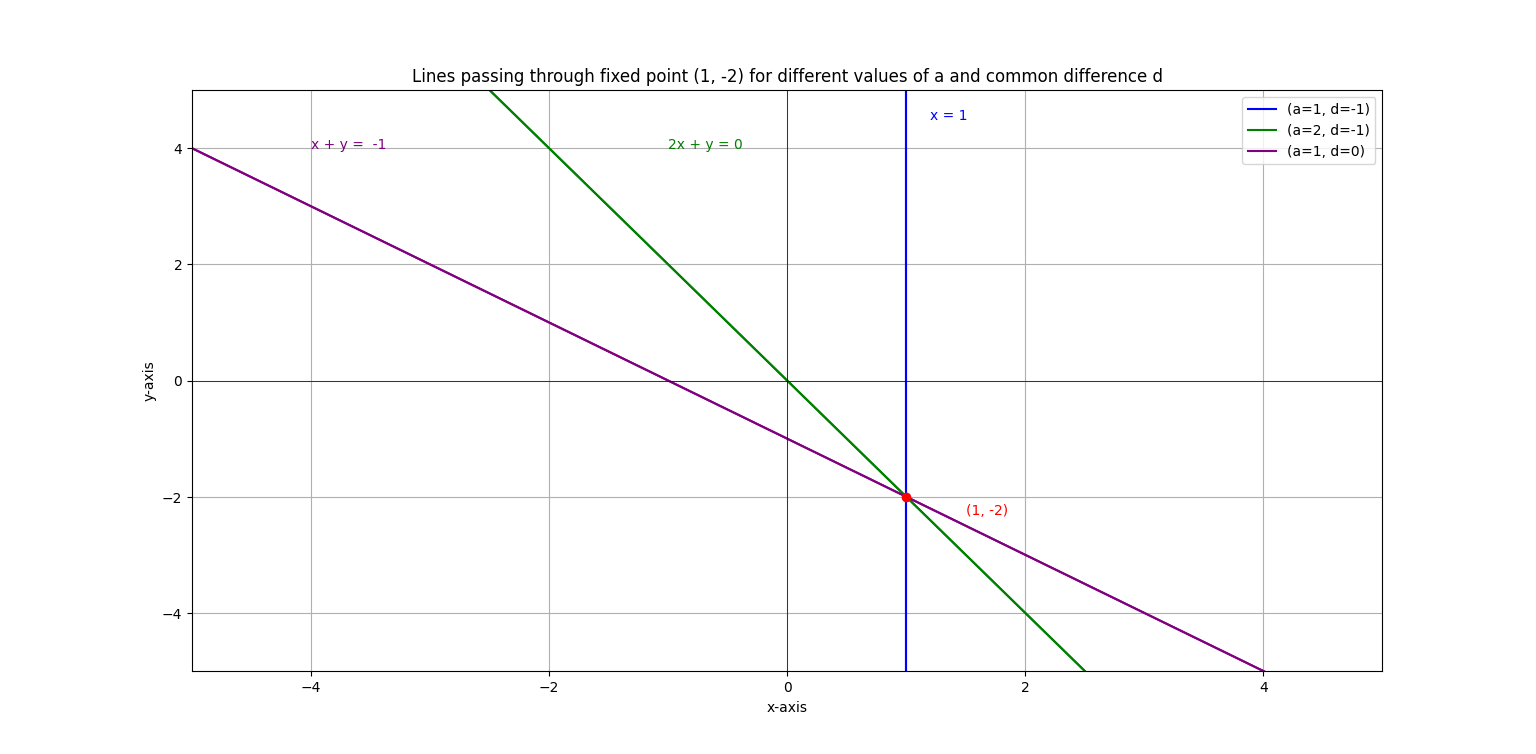
\includegraphics[width=0.9\columnwidth]{../figs/figure_py.png}
        \caption{Line passing through a fixed point}
        \label{fig:final_plot}
    \end{figure}
\end{frame}
\end{document}
